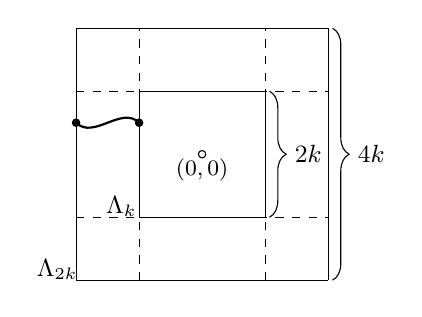
\begin{tikzpicture}[scale = 0.4]

	\draw[solid, black] (-2, -2) -- ( 2, -2);
	\draw[solid, black] ( 2, -2) -- ( 2,  2);
	\draw[solid, black] ( 2,  2) -- (-2,  2);
	\draw[solid, black] (-2,  2) -- (-2, -2);
	
	\draw[solid, black] (-4, -4) -- ( 4, -4);
	\draw[solid, black] ( 4, -4) -- ( 4,  4);
	\draw[solid, black] ( 4,  4) -- (-4,  4);
	\draw[solid, black] (-4,  4) -- (-4, -4);
	
	\draw[dashed, black] (-2, -4) -- (-2, 4);
	\draw[dashed, black] ( 2, -4) -- ( 2, 4);
	\draw[dashed, black] (-4, -2) -- ( 4,-2);
	\draw[dashed, black] (-4,  2) -- ( 4, 2);
	
	\draw[black] ( 0,  0) circle (3.35pt);
	\node[black] at (0, -.5) {{\footnotesize $(0, 0)$}};
	\node[black] at (-2.4, -1.65) {{\small $\Lambda_{k\phantom{2}}$}};
	\node[black] at (-4.6, -3.65) {{\small $\Lambda_{2k}$}};
	
	\draw[fill] ( -2,  1) circle (3.35pt);
	\draw[fill] ( -4,  1) circle (3.35pt);
	
	\draw[solid, thick, black] (-2, 1) to[out = 135, in = -45] (-4, 1);
	
	\draw [decorate, decoration = {brace, amplitude = 6pt, mirror}, xshift = 4pt, yshift = 0pt] (2, -2) -- (2, 2) node [black, midway, xshift = 14pt, yshift = 0pt] {\small $2k$};
	
	\draw [decorate, decoration = {brace, amplitude = 6pt, mirror}, xshift = 4pt, yshift = 0pt] (4, -4) -- (4, 4) node [black, midway, xshift = 14pt, yshift = 0pt] {\small $4k$};
	
\end{tikzpicture}